  \chapter{Fundamentação} \label{cap:teoria}
  
Este capítulo apresenta a fundamentação necessária para a compreensão e desenvolvimento desta pesquisa. Especificamente, os seguintes tópicos são revisitados: Análise de dados e Redes Neurais Artificiais.
 
% ----------------------------------------------------------
% TEORIAS PARA PRE PROCESSAMENTO DOS DADOS
% ----------------------------------------------------------
\section{Análises dos Dados}

A análise de dados é um processo bastante amplo. Essa tarefa visa tratar os dados desde sua aquisição e pré-processamento até a sua interpretação a partir de ferramentas complexas de mineração. Essa seção inicia com a apresentação dos tipos de dados considerados nesse projeto. Na sequência, alguns aspectos sobre a análise exploratória de dados, definições sobre séries temporais e métodos de predição são brevemente introduzidos.

\cite{Junior2007} realiza um trabalho amplo de análise de diversos métodos de previsão de demanda, e cita que dados coletados em modelos de previsão possuem informações que quando são projetadas graficamente evidenciam comportamentos que em alguns casos podem ser visualizados e generalizados de forma subjetiva pelos gestores dos dados. Em todos os casos, a análise de dados é necessária para selecionar parâmetros de demanda que contribuem de forma positiva à uma predição.

Também cita que somente a análise de dados não é o suficiente e que se realizada nos intervalos ou critérios incorretos pode comprometer seriamente as conclusões do comportamento dos dados, e que por sua vez pode comprometer seriamente a decisão dos gestores responsáveis por estes dados, no cenário de uma previsão de demanda.  Isto ocorre atualmente no cenário de previsão da demanda de refeições do ICT-UNIFESP, onde a universidade e o estabelecimento que fornece as refeições não informa nenhum modelo de previsão de demanda ou expõe alguma análise de dados que possam influenciar na demanda de consumo do restaurante. 

Como foi evidenciado nas comunicações com a gestão do restaurante, a análise utilizada para se prever as refeições é produzir no dia da semana, como por exemplo uma segunda-feira, o consumo do mesmo dia da semana anterior (segunda-feira anterior) com acréscimo de uma margem de erro. Em geral, de acordo com o restaurante, todos os dias o mesmo trabalha com um erro e um descarte de 30\% das refeições que são trazidas e consumidas ao campus. Estima-se então que no período de 2011 - 01/08/2018 os estabelecimentos tenham tido um prejuízo de R\$1.885.938,40, e de 30\% de R\$78.386,85 no atual período de 01/08/2018 - 31/10/2018 totalizando o montante  R\$1.964.325,25. Aproximadamente 2 milhões de reais em prejuízo acumulado desde 2011.

\subsection{Tipos de dados}
  
Este trabalho denomina 2 tipos de dados contemplados nas predições e seus parâmetros: 
Endógenos e Exógenos. Ambos são detalhados a seguir:
            
\paragraph{Endógenos}
Dados endógenos são os dados do domínio de predição, neste caso, são os valores de consumo de refeições representado pela quantificação da passagem dos alunos no ponto de acesso, a catraca, do restaurante universitário do ICT Unifesp.
São considerados endógenos também os dados de consumo de jantar, e os dados de vendas de tickets de refeições, todos discretizados e somados por dias letivos. Além disso, neste trabalho, os dados endógenos são transformados em entrada das redes neurais, em formato de série temporais, fundamentada nas seções adiante.
            
\paragraph{Exógenos}
Os dados exógenos são todos os outros dados fora do domínio de predição, incluso parâmetros derivados das datas das observações como por exemplo o dado categórico que representa o dia da semana (segunda-feira à sexta feira), outros dados que derivam da data dos registros dos dados endógenos e por fim os dados climáticos.
          
          
\subsection{Séries Temporais}

\TODO{Essa seção poderia definir formalmente uma série temporal (equação).}

De acordo com  \cite{Morettin1987}, uma série temporal é um conjunto de observações ordenadas em função do tempo, comumente iguais, apresentando uma dependência serial entre elas, sendo um dos objetivos do estudo de séries temporais, analisar e modelar essa dependência. Além disso, séries temporais são analisadas pelos seus principais movimentos, como tendência, sazonalidade e a componente aleatória, sendo a tendencia e sazonalidade as propriedades que mais ganham destaque em pesquisas de previsão de demanda de carga elétrica.

A obtenção dos dados do R.U do ICT Unifesp se encontra em formato de série temporal, ou seja, o consumo e vendas de refeições no R.U se distribuem em função do tempo, pelos dias letivos da universidade.

Almeida \cite{Almeida2013} em sua análise afirma que para realizar a previsão de uma determinada série temporal é possível utilizar diferentes métodos. Pode-se classificá-los basicamente entre métodos estatísticos e métodos baseados em inteligência artificial. Sendo abordado neste trabalho os métodos de redes neurais artificiais contemplados na disciplina de inteligência artificial.
  
É importante observar que os métodos de previsão em séries temporais buscam uma redução da série temporal à um modelo estacionário e a decomposição da série em componentes de tendência, ciclo, sazonalidade e termo aleatório. A tendência entende-se pelo movimento persistente dos dados em uma direção, o ciclo indica o movimento oscilatório desta tendência, sazonalidade indica comportamento regular assumido de forma repetitiva e o termo aleatório se dá por movimentos irregulares presentes na série.

 %\TODO{CITAR CORRETAMENTE}
WOOLDRIDGE, Jeffrey M. Introductory Econometrics: a Modern Approach. 2000, South-Western College Publishing, a division of Thomson Learning. ISBN 0-538-85013-2. Capítulo 1, Página 8, formaliza e descreve os componentes de uma série temporal, conforme a tabela \label{table:componentes_serie_temporal}.
           
As técnicas de previsão para evidências sazonais, usam métodos de regressão, que podem ser observados nos trabalhos de previsão de consumo de energia elétrica realizados pelas pesquisas de \cite{Almeida2013}, \cite{RUAS2012} e de \cite{Silva2010}, além , da previsão de demanda de produtos cosméticos pelo trabalho de \cite{Junior2007}

O cenário deste estudo analisa a sazonalidade da frequência de alunos do ICT - UNIFESP, inferida pelas grades semestrais de suas disciplinas, que consequentemente inferem na sazonalidade de consumo de refeições dentro do restaurante universitário.\newline

\subsection{Métodos de Previsão de Demanda} 

A previsão de demanda pode ser definida como um processo de busca de informações que geram vendas de um produto ou um conjunto de produtos.

O autor \TODO{Citar e incluir o autor, MOREIRA, Daniel Augusto. Administração da produção e operações. São Paulo: Editora Thomson Learning, 2002.} cita que os métodos de previsão de demanda são os processos que utilizam tais informações para definir uma demanda futura destes itens, desde métodos subjetivos e intuitivos até métodos matemáticos e computacionais, classificado os modelos de previsão em dois grandes grupos: métodos qualitativos e métodos quantitativos.

No trabalho de \cite{Junior2007}, ilustrado na figura \label{fig:metodosPrevisaoDemanda}, os métodos qualitativos são definidos como um julgamento dos dados expostos sem um sistema de processamento analítico para se produzir novos modelos ou dados, sendo úteis para sistemas de agrupamento, clusterização ou classificação de dados, sem fornecer novas informações numéricas ou modelos preditivos. Já os métodos quantitativos, sendo o foco deste trabalho, são definidos como analíticos e se baseiam em um modelo matemático para realizar previsões. Para realizar tais previsões os métodos quantitativos necessitam de um histórico de dados, para analisar padrões em seu comportamento e predizer o futuro que irá agir dentro deste padrão.

          \begin{figure}[H]
          	\center{
          	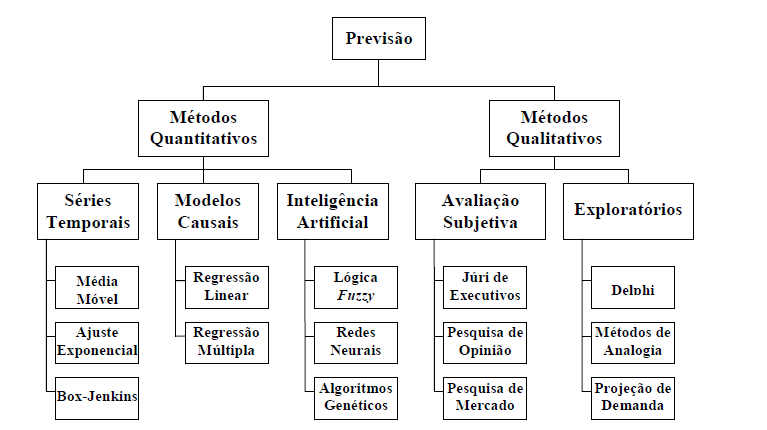
\includegraphics[width=0.65\textwidth]{./Figs/02-junior-metodos-previsao-demanda.png}
          	\caption{Métodos de previsão de demanda. Fonte: \cite{Junior2007}.}
          	\label{fig:metodosPrevisaoDemanda}}
          \end{figure}

E conforme a figura \ref{fig:metodosQuantitativos},} estes métodos se ramificam em 2 tipos, as séries temporais e os modelos causais.

          \begin{figure}[H]
          	\center{          		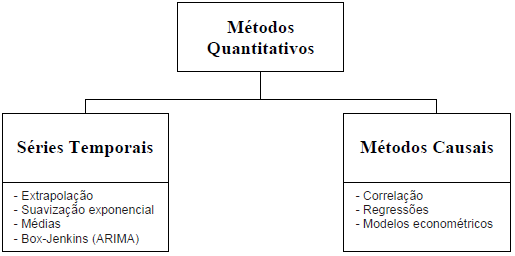
\includegraphics[width=0.65\textwidth]     		{./Figs/01-junior-metodos-quantitativos.png}
          	\caption{Tipos de métodos quantitativos. Fonte: \cite{Junior2007}}.
          	\label{fig:metodosQuantitativos}}
          \end{figure}

O comportamento dos dados deste trabalho, apesar de ter uma distribuição de datas em função do tempo se classificando em um modelo de série temporal, assume-se a hipótese que tem tal comportamento impactado por relações causais com outras variáveis como recesso acadêmico, feriados, eventos, precipitações intensas que causam trânsito local e impactam na logística e frequência do público, entre outras variáveis de causas menos aparentes.


          
Na figura \ref{fig:seriesTemporais} temos um exemplo de sazonalidade diária de dados.

\TODO{o comando subcaption* nas figuras está acarretando na numeração incorreta. Veja o que fiz nas figuras anteriores e replique para as demais}

          \begin{figure}[H]
          	\center{
          		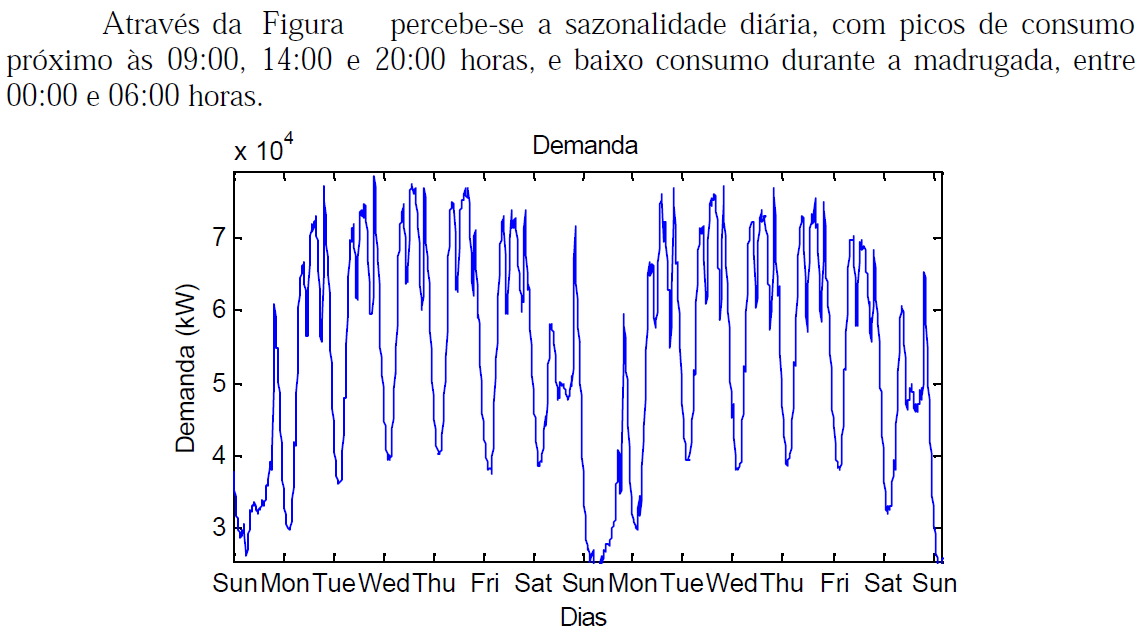
\includegraphics[width=0.65\textwidth]{./Figs/03-ruas-serie-temporal-sazonal.png}
          	
          	\caption{Dados de demanda de sazonalidade diária, em função do horário.} \subcaption*{ Fonte: \cite{RUAS2012}}.\label{fig:seriesTemporais}}
          \end{figure}

\TODO{Reorganizar as Subseções abaixo. Vou renomear a Seção principal como Redes Neurais, internamento, introduzimos IA.}


\section{Redes Neurais Artificiais}

\TEXTO{As redes neurais são ... (definir e CITAR o livro do Haykin).... As redes neurais fazem parte da grande área de conhecimento denominada Inteligência Artificial (IA) CITAR}

% \subsection{Inteligência Artificial}

% "A inteligência artificial é o ramo da ciência da computação que se ocupa do comportamento inteligente." \cite{Luger2004}.
% O termo "Inteligencia Artificial" surgiu em meados de 1956 em uma conferência, chamada Dartmouth Summer Research Project on Artificial Intelligence, sediada nos Estados Unidos em Dartmouth College, Hanover, New Hampshire, a conferência foi organizada por John McCarthy e teve como proposta reunir matemáticos, cientistas da computação e pesquisadores buscando meios de como fazer com que as máquinas usem linguagem, abstrações de formulários e conceitos, para resolver problemas que eram reservados aos humanos, e que consigam melhorar o seu próprio desempenho.

Sistemas de inteligência artificial buscam então resolver funções e problemas que seres humanos conseguem resolver melhor do que máquinas convencionais, usando sua capacidade de abstração e aprendizagem com o erro.

\TEXTO{A inteligência artificial é o ramo da ciência da computação que se ocupa do comportamento inteligente." \cite{Luger2004}. Sistemas de inteligência artificial buscam então resolver funções e problemas que seres humanos conseguem resolver melhor do que máquinas convencionais, usando sua capacidade de abstração e aprendizagem com o erro. De uma forma geral, a IA pode ser dividida em diversas subcategorias, a descrição completa de todas as subcategorias está fora do escopo deste trabalho. O restante dessa seção irá se concentrar no tema Redes Neurais.}

\subsection{Neurônio Artificial}
         
        %   \paragraph*{História e inspiração da Inteligência Artificial}
            %Redes Neurais Artificiais são elementos de inteligência artificial da ciência da computação, inspirados no funcionamento do cérebro humano.

\TEXTO{A unidade básica de uma rede neural artificial é o neurônio (CITAR)}. \TODO{Esse paragrafo está falando sobre RNAS e não Neurônios, poderia subí-lo para o inicio da Seção} Assim, as redes são formadas por neurônios artificiais interconectados que são capazes de processar múltiplos valores de entradas, e reagir produzido uma resposta relacionada à essas entradas. Como qualquer outro método de aprendizado de máquina, este modelo busca obter um aprendizado a partir dos dados de entrada recebidos, criando uma capacidade de generalização de problemas e assim buscam o objetivo principal de resolver novos problemas com este aprendizado.

\TODO{IDEM para esse paragrafo}Uma rede neural pode não produzir uma resposta esperada, resolvendo erroneamente um problema, assim como o cérebro humano tem limitações de aprendizado, que levam o homem a cometer falhas de decisões ou ações por um aprendizado mal treinado. Por isso as características fundamentais que tornam uma rede neural artificial em uma boa solução, é um bom planejamento de sua topologia, e método de treinamento, que serão explicados a seguir.

%\cite{Muhammad2014} demonstra que a propriedade fundamental do cérebro é a sua capacidade de mudar com uma grande variedade de experiências, inclusive lesões que provocam perdas de neurônios, abordando princípios de plasticidade cerebral, mostra também que a capacidade de aprendizado de mamíferos que sofreram uma redução de neurônios causada por lesões, pode ser restaurada não somente pela recuperação desses neurônios perdidos, mas sim por novas conexões e sinapses entre outros neurônios. Ou seja, a rede sofre uma mudança de topologia.

%\cite{Fapesp192} Mostra em um experimento recente que o cérebro humano possui atualmente 86 bilhões de neurônios interconectados, e que sua capacidade de aprendizado e habilidades evolutivas também vêm aumentando em conjunto com seu número de neurônios e topologia de rede neural, que há 30 milhões de anos atrás tinha apenas 2,5 bilhões de neurônios e era apenas um animal arborícola quadrúpede.

          \paragraph*{Neurônio Biológico}
            O modelo de neurônio artificial surge então, com a busca da inteligência artificial de reproduzir o comportamento de aprendizado humano, reproduzindo computacionalmente seu elemento biológico principal de aprendizagem: O neurônio biológico. 
            \begin{figure}[H]
              \center{
                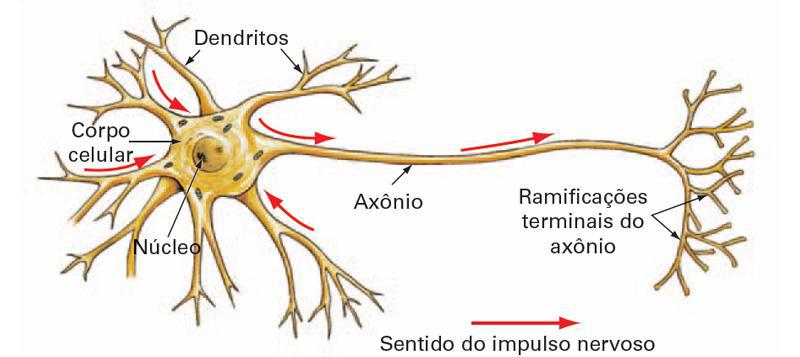
\includegraphics[width=0.65\textwidth]
                {./Figs/05-neuronio.jpg}
              
              \caption{Neuronio Biológico} \subcaption*{Fonte:  https://pt.khanacademy.org/science/biology/human-biology/\\neuron-nervous-system/v/anatomy-of-a-neuron.}\label{fig:NeuronioBiológico}}
            \end{figure}

Um neurônio biológico figura \ref{fig:NeuronioBiológico} trata as informações recebidas por meio de seus dentritos e processa-as em seu corpo celular, tal reação à esses estímulos recebidos gera um sinal de saída como resposta aos estímulos, enviado através do axônio. Esse estímulo é repassado como sinal de entrada, através de outros neurônios por meio de seus dendritos, e o ciclo se repete em uma vasta rede.
Controlando essas conexões, pontos de contato entre a resposta de um neurônio e a entrada de outro, existem as sinapses. Elas funcionam como agentes que permitem a interação acontecer ou inibem, e são acionadas por um conjunto somatório de estímulos. Se tal somatório de estímulos for satisfatório, elas permite a transmissão de sinal elétrico pelo axônio até o dendrito de um neurônio vizinho, formando um ciclo de aprendizado em uma rede neural biológica.

        %   \paragraph*{Neuronio Artifical - MCP}
Warren McCulloch e Walter Pitts em 1942 observando o neurônio biológico iniciam a busca de um modelo computacional do mesmo. McCuloch era psiquiatra e neuroanatomista e passou cerca de 20 anos refletindo e estudando sobre a representação do sistema nervoso, em 1942 ele convidou Pitts, que era matemático, para fazer parte das suas pesquisas. Em 1943 lançaram o artigo "A Logical Calculus of the Ideas Immanent in Nervous Activity." chegando em um modelo matemático do neurônio artificial: 

            \begin{figure}[H]
                \center{
                  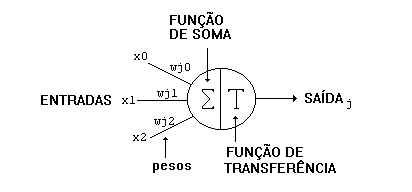
\includegraphics[width=0.65\textwidth]
                  {./Figs/06-neuronio-artificial.png}
               
                \caption{Neuronio Artificial.} \subcaption*{ Fonte: \url{http://redesneuraisartificiais.blogspot.com/2010/10/o-primeiro-modelo-de-um-neuronio-criado.html}} \label{fig:NeuronioArtificial} }
            \end{figure}

Assim como no neurônio biológico, o modelo de neurônio artificial da figura \ref{fig:NeuronioArtificial} reage à um vetor de entradas $x_0$ à $x_2$ onde tem suas sinapses representadas por pesos numéricos $wj_0$ à $wj_2$, com uma soma ponderada dessas entradas que é controlada por uma função de transferência ou função de ativação, determinando se essa soma é maior que um valor numérico. Se essa soma for satisfatória o neurônio é ativado emitindo um valor de saída 1, caso contrário se emite um valor de saída 0.
Todo o funcionamento deste modelo então é reduzido a responder se a soma recebida é maior que um valor numérico esperado. Contudo, associado a este neurônio não foi proposto uma forma automática para ajuste dos pesos, ou seja, não há um algoritmo de aprendizagem \cite{Haykin1994}.
        
\subsection{O Perceptron}
        %   \paragraph*{Perceptron}

O modelo de Warren McCulloch e Walter Pitts, apesar de conseguir simular o modelo de neurônio biológico e resolver algumas tarefas lógicas e matemáticas não atendia o objetivo principal da Inteligência Artificial: A capacidade de aprendizado.
Para utilizar um modelo de neurônio artificial a fim da solução de um problema era necessário conhecer o ajuste dos pesos das entradas, e em uma tarefa de um cenário complexo e com muitas variáveis, ou pesos não perceptíveis ao valor esperado de saída, o ajuste não se torna trivial.
            
Em 1958, o cientista da computação Frank Rosemblatt desenvolveu o primeiro modelo de rede neural artificial com um algoritmo de aprendizado para o neurônio MCP, denominada de Perceptron, para solucionar este problema de ajuste de pesos.
Basicamente neste novo modelo, os pesos das conexões são ajustados de forma autônoma com a introdução de pessoas associados e um valor bias, a fim de buscar um reconhecimento autônomo de padrões. Tarefas de reconhecimento de padrões simples com separações lineares os seres humanos conseguem realizar de forma trivial mas ainda era um desafio para tal problema se resolvido por uma máquina.
            
            Então em 1969, Marvin Mjinsky e Seymour Papert realizaram uma publicação comprovando essa limitação de aprendizado à uma combinação linear, e provaram que o perceptron é limitado à resolução de problemas que são resolvidos ou classificados por apenas 1 linha, ou seja, problemas linearmente separáveis que consiste na mesma limitação do processo de regressão linear múltipla.
            
            Na figura \ref{fig:problemasLineares} o perceptron não pode solucionar o problema (b). E essa limitação desmotivou e parou os estudos com perceptrons.
    		  \begin{figure}[H]
    		  	\center{
    		  		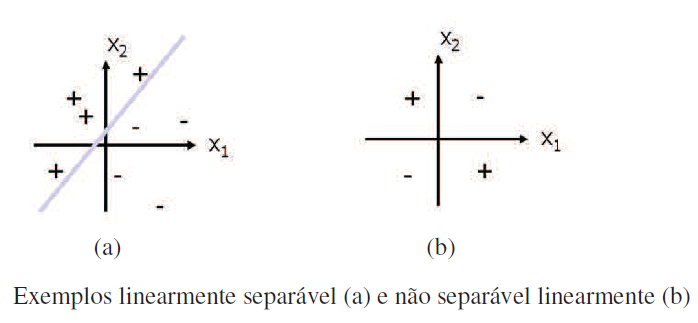
\includegraphics[width=0.65\textwidth]
    		  		{./Figs/10-limite-perceptron.png}
    		  
    		  	\caption{Problemas Linearmente Separáveis e Não Separáveis.} \subcaption*{Fonte: \cite{Flavia2014}.}\label{fig:problemasLineares}}	
    		  	
    		  \end{figure}
	  	
	  	    Em 1986 James McClelland e David Rumelhart proporam o método de desenvolvimento de uma rede neural de perceptrons, tangendo mais ainda a inspiração da solução no cérebro humano. O processo resume o treinamento do perceptron simples aplicado à um conjunto de perceptrons interligados, e assim solucionando problemas complexos que podem ser resolvidos com uma combinação de soluções.
	  	  
  	  	  \begin{figure}[H]
  	  	  	\center{
  	  	  		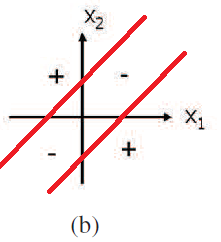
\includegraphics[width=0.30\textwidth]
  	  	  		{./Figs/11-solucao-mlp.png}
  	  	  	
  	  	  \caption{Problemas Linearmente Não Separáveis. Múltiplas Soluções.}  \label{fig:doisPerceptrons}}
  	  	   \end{figure}

            A rede perceptron , conforme demonstrado no trabalho de\cite{Flavia2014}, possui apenas uma camada de entrada e saída, a saída utiliza como função de ativação a função degrau $ \delta(.) $ que define quando o neurônio emitirá o sinal lógico 1 ou quando emitirá o sinal lógico 0.

            O sinal de saída do perceptron entende-se então por:
            $y_j= \delta(\sum_{i=1}^{n}x_i W_{ji}+b_j)$
            \begin{itemize}
            	\item $ x_i $ - sinais de entrada do neurônio;
            	\item $ w_{ji} $ - pesos sinápticos do neurônio;
            	\item $ b_j $ - bias ou limiar de ativação;
            	\item $ \delta(.) $ - função de ativação;
            	\item $ y_j $ - sinal de saída do neurônio.
            \end{itemize}
			
            \begin{figure}[H]
            	\center{
              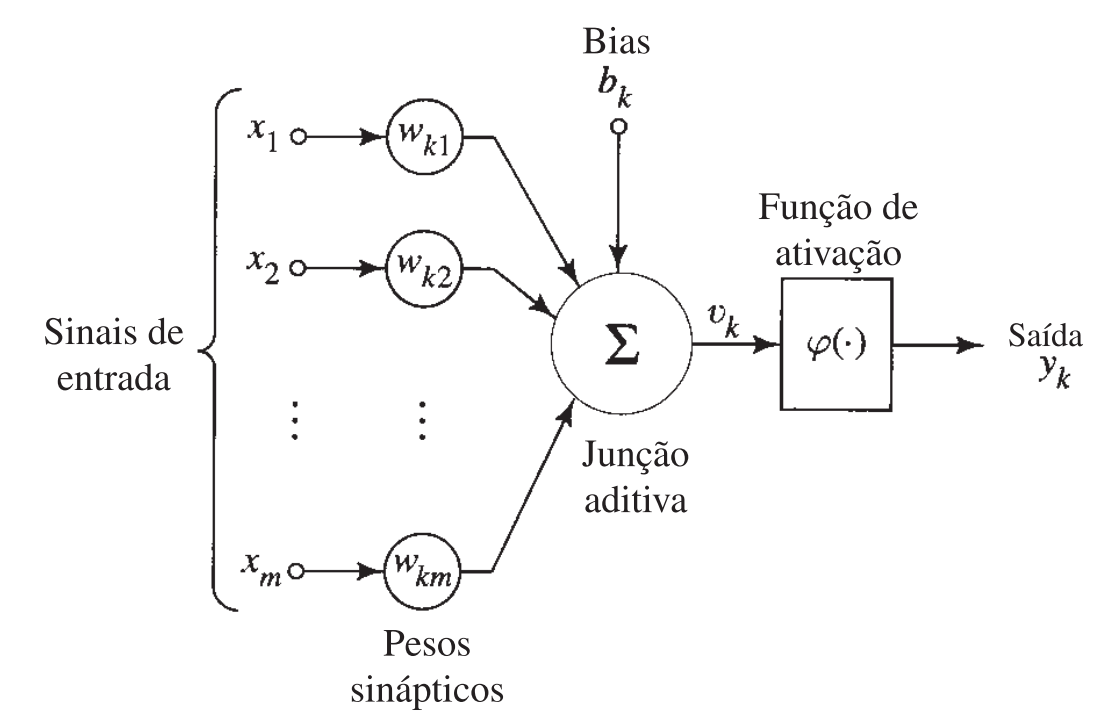
\includegraphics[width=0.65\textwidth]
              {./Figs/08-perceptron.png}
           
            \caption{Neurônio Artificial Perceptron.} \subcaption*{ retirado de \cite{Junior2007}} \label{fig:perceptron} }
            \end{figure}
			
		     Em algumas literaturas o bias pode ser reduzido a um peso $W_0$ com entrada $X_0$ fixo em 1 no neurônio, a representação gráfica da topologia pode mudar, mas no somatório de saída, o calculo continua o mesmo.
		
		     A função de ativação $\delta$ se apresenta de forma linear ou não linear, determinando a saída de um neurônio a partir do seu potencial de ativação. 
		
		     \begin{figure}[H]
				\center{
					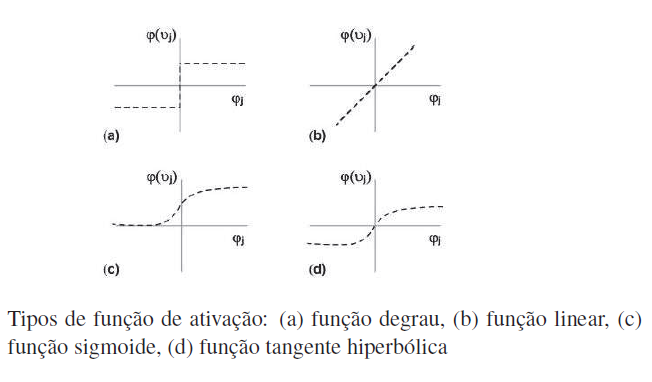
\includegraphics[width=0.80\textwidth]
					{./Figs/09-delta.png}
				
				\caption{Funções de Ativação.} \subcaption*{ Fonte:  \cite{Flavia2014}: \label{fig:perceptron2}}}
		     \end{figure}
		
		     A função de ativação dá a capacidade do perceptron. quando conectado em rede, de resolver problemas lineares e não lineares, agregando adaptação e improviso ao resolver programas que não estão contidos em seus dados de alimentação.
			
		  %\paragraph*{Perceptron - Treino Supervisionado}
\cite{Almeida2013} cita em sua análise que o processo de aprendizado do perceptron pode ocorrer de forma supervisionada quando o neurônio deve aprender a relacionar um conjunto observado de variáveis à um valor observado de saída deste mesmo conjunto. O neurônio recebe os sinais de entrada $Xi$ e produz uma saída $Yi$ através do combinador linear e função $\delta$ de ativação; compara essa saída $Yi$ com a observação $i$ obtida do conjunto de dados (ponto chave do processo de treino supervisionado) e por fim essa comparação irá gerar um erro $e$.
            
            % \subparagraph*{Critério de parada}
De acordo com algum critério adotado em cada contexto de aplicação do perceptron, este erro pode ser aceitado e o neurônio mantém o valor de seus pesos $Wi$ que impactam na saída $Yi$ desejada. A aprendizagem do neurônio também pode atingir um critério de parada após N épocas de treinamento, diversos critérios de paradas  podem ser combinados.  
            	
            % \subparagraph*{Época de treinamento}
Se o critério de parada não for aprovado, uma nova época de treinamento (ou repetição de interação) é iniciada mesmos valores $X_i$ e $Y_i$ passados, os valores de pesos $Wi$ são reajustados com a taxa de aprendizagem, buscando o objetivo de se obter um erro menor.
            	
            % \subparagraph {Taxa de aprendizagem}
Esse reajuste de pesos $Wi$ denomina-se taxa de aprendizagem, $\alpha$ que pode ter valores de escolha livre ao contexto de aplicação do perceptron, para reajustar estes pesos $Wi$. Assim que a taxa de aprendizagem ajusta os pesos, uma nova época N+1 de treinamento está se iniciando buscando novamente um erro menor. Ressaltando então que o critério de parada pode ser acionado e interromper o reinicio do processo, se for estipulado um limite para o valor de N combinado ou não com um limite para o erro. 
            	
  	    %%%%%%%%%%%%%%%%%%%%%%%%%%%%%%%%%%%%%%%%%%%%%%%%%%%%%   
\subsection{Rede Perceptrons Múltiplas Camadas - MLP}
  	       
  	       A solução base para se combinar 2 ou mais camadas de perceptrons a fim de se resolver um problema com a combinação de 2 ou mais soluções lineares, é a utilização de um perceptron combinador de sinal de saída, já que cada perceptron pode ter múltiplas entradas e somente uma saída. Dessa forma as redes neurais vão formando colunas de perceptrons interconectados. Cada coluna é denominada uma camada da rede neural. A ultima camada deve ter o número de perceptrons correspondente ao número de saídas desejadas. Na figura abaixo, encontra-se uma rede neural com duas camadas intermediárias e 3 saídas.
  	       
  	       \begin{figure}[H]
  	       	\center{
  	       		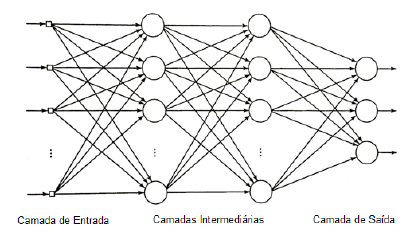
\includegraphics[width=0.65\textwidth]
  	       		{./Figs/12-mlp.png}
  	       	
  	       	\caption{Rede de perceptrons com múltiplas camadas.} \subcaption*{Fonte: \cite{Almeida2013}}\label{fig:MLP}}
  	       \end{figure}
         
  	       Esta rede denominada MLP (Multilayer Perceptron) possui uma camada de entrada onde cada nó representa uma variável a ser considerada ao problema a ser analisado, e pelo menos uma camada intermediária.
  	      
  	       Nesta camada intermediária os neurônios possuem geralmente uma função de ativação sigmoidal logística ou tangente hiperbólica, e conceitualmente no mínimo 1 neurônio desta primeira camada oculta deve receber no mínimo 2 conexões de entrada. E uma camada de saída, na borda à direita, com o número de neurônios correspondente ao número de soluções buscadas. 
  	       
            % \paragraph*{Treino e Validação da MLP}
            	O conjunto de dados de entrada na rede MLP supervisionada, deve ser dividido em 2 partes principais, Treinamento e Validação. É importante salientar que as observações de ambos os conjuntos devem originar do mesmo conjunto de dados para representar o mesmo problema, as observações $Y_i$ relacionadas aos vetores $i$ de variáveis $X_{i1},Xi_{i2},...,X{ij}$ do conjunto de treino, devem ter a mesma estrutura, mesmo número j de variáveis X por vetor de entrada e devem representar o mesmo problema que as observações $Yi$ do conjunto de validação.
            	
            	O conjunto de dados da validação e treino somados devem formar exatamente o conjunto original, sem informações excedentes ou em falta.
            	
            	Os dados de treino e dados de validação, podem ser separados de forma aleatória, sendo os dados de treino os responsáveis pelos reajustes de pesos e capacidade de generalização da rede, e os dados de validação responsáveis pelo processo de validação pós-treino.
            	
            	É importante adotar um bom critério de parada de treino, pois um treino prolongado tende a convergir em ajustes de pesos memorizados dos valores observados nos dados de treino e isso causa o fenômeno de overfitting na rede neural, que é a perda da capacidade de generalização. Pesos sinápticos que sofrem processo prolongado de reajustes acaba "viciando" a rede neural para reconhecer apenas os dados de treino.
            	
            % 	\subparagraph{ Parada do erro mínimo:}
            	O critério de parada do erro mínimo encerra o treinamento da RNA quando a mesma obtém um erro menor que o mínimo estipulado para o valor observado, este é o critério mais simples, adotado nos casos onde existe um limiar de erro já determinado pelo problema, entre o valor observado e o valor a se predizer.
            	
            % 	\subparagraph{Parada por número de épocas:}
            	Um critério de parada pode ser limitado também ao número de épocas de treino. A determinação  deste número de épocas pode ocorrer por tentativa e erro, visto que haverá a convergência de um número pequeno para uma baixa capacidade de aprendizado, e a convergência de um número grande para o processo de overfitting. Logo é necessário realizar experimentos que validem número de épocas fora desses intervalos de convergência.
            	
            % 	\subparagraph{Parada por validação cruzada:}
            	Por fim a validação cruzada é a técnica que se utiliza os dados dos conjuntos de validação e treino de forma cruzada, neste processo então, os dados de treino são utilizados no processo interativo de aprendizagem, e no fim deste processo o conjunto é validado com os dados de validação, obtendo-se um novo erro de validação.
            	A medição do erro de validação passa por um processo de avaliação em função do número de épocas, a fim de se detectar um ponto de número de épocas onde o erro quadrático médio da amostra de validação sofre uma curva de crescimento após um limiar de decréscimo.
            	
            	É notório observar que o erro quadrático médio das amostras de treinamento sofrerá um decréscimo em função do aumento do número de épocas de treinamento, convergindo ao processo de overfitting, ou memorização da rede.
            	
            	O ponto de parada no limite inferior do erro quadrático médio da amostra de validação, será o ponto ótimo de parada de treinamento.
          	
          	\begin{figure}[H]
          		\center{
          			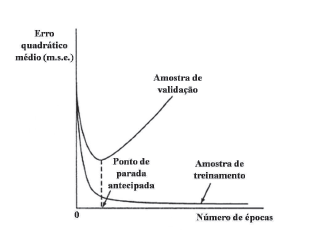
\includegraphics[width=0.5\textwidth]
          			{./Figs/14-validacaocruzada.png}
          		
          		\caption{Ponto ótimo de parada da validação cruzada.} 
          		\subcaption*{ Retirado de \cite{Flavia2014}} \label{fig:validacaoCruzada}} 
          	\end{figure}
        
        % O treinamento de uma rede MLP para previsões de demanda de restaurantes universitários que obteve sucesso em \cite{Lopes2008} e \cite{Rocha2011} é a retro propagação de erro.
        %%%%%%%%%%%%%%%%%%%%%%%%%%%%%%%%%%%%%%%%%%%%%%%%%%%%%%%%%%%%%%%%%%%%%%%

\subsection{O Algoritmo de Retro Propagação \textit{Backpropagation}}

        A rede Perceptron Múltiplas Camadas com Retro Propagação de Erro (do inglês, M.L.P Backpropagation), faz o reajuste dos pesos sinápticos dos neurônios através de duas fases:
  	       \paragraph*{Feed-forward} Nesta primeira fase de treino os sinais $X_{i0},X_{i0},...,X_{in}$ com sua respectiva saída $Y_i$ do conjunto de dados são apresentados à todos os neurônios da primeira camada. O processo de propagação do sinal de saída de cada neurônio segue o princípio do neurônio artificial apresentado na seção anterior, que envia o sinal de saída como um sinal de entrada ao neurônio seguinte.
  	       
  	       \paragraph*{Feed-backward} Nesta fase é obtido um valor de erro da camada de saída. Este erro é utilizado na equação de reajuste do peso sináptico das conexões dos neurônios da camada de saída com o sinal de saída dos neurônios da última camada oculta. E depois este erro é propagado realizando outra equação de reajuste de peso sináptico das conexões dos neurônios nas camadas anteriores, no sentido contrário em direção à camada de entrada. Isto permite que os pesos sináptico de todas as camadas de intermediárias neste processo tenham seus pesos ajustados.
  	       
  	       \begin{figure}[H]
  	       	\center{
  	       		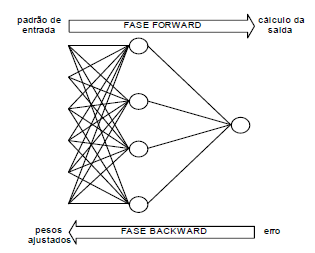
\includegraphics[width=0.65\textwidth]
  	       		{./Figs/13-mlp-back.png}
  	       	
  	       	\caption{Fases de treino da MLP-Back-Propagation.} \subcaption{Fonte:  \cite{Almeida2013}}\label{fig:MLP2}}
  	       \end{figure}
  	       
  	       \paragraph*{MLP Backpropagation em R.U em trabalhos relacionados}
  	       De acordo com  o trabalho de \cite{Lopes2008}, a rede neural perceptron de múltiplas camadas é utilizada para tratar a previsão de demanda do R.U da UFV, utilizando apenas como variáveis quantitativas as 5 ultimas observações anteriores ao dia a se analisar, e como variáveis qualitativas o dia da semana variando de segunda a sexta, em valores binários.
  	       
           \begin{figure}[H]
          	\center{
          		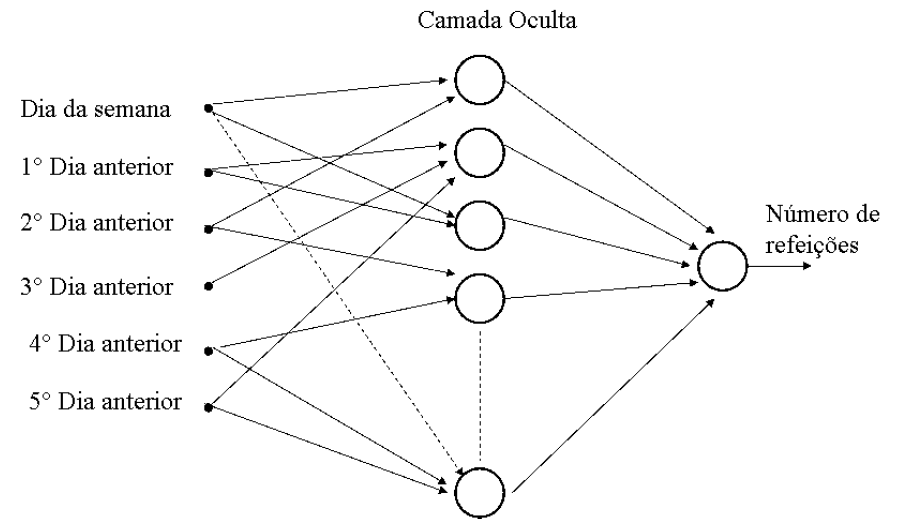
\includegraphics[width=0.65\textwidth]
          		{./Figs/15-rna-lopes.png}
          	
          	\caption{Rede Neural Perceptron de Múltiplas Camadas.} \subcaption*{ Fonte:  \cite{Lopes2008}.}\label{fig:mlp-lopes}}
           \end{figure}
            
           Conforme  o trabalho realizado por  \cite{Rocha2011} com neurônios artificiais para prever a demanda do R.U da UNESP, envolve apenas uma única camada de entrada e uma segunda camada para saída, porém com uma diversidade maior de variáveis de entrada correlacionadas com o consumo do restaurante. 
           \begin{figure}[H]
          	\center{
          		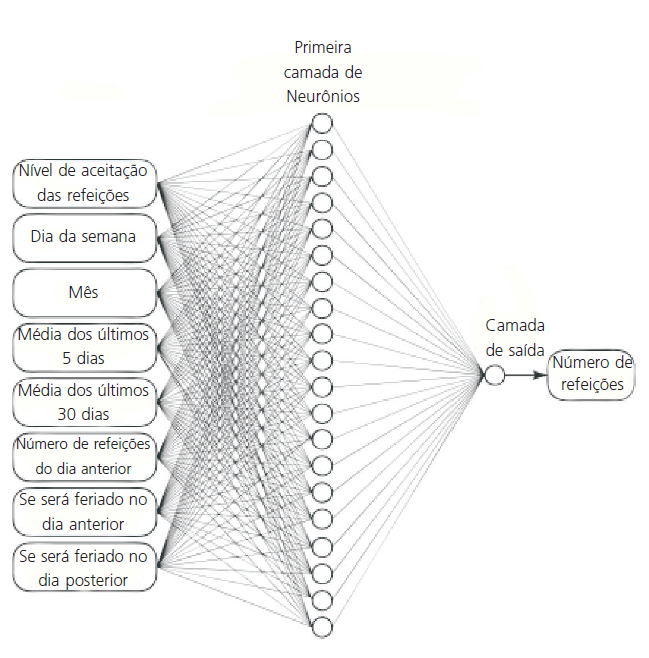
\includegraphics[width=0.65\textwidth]
          		{./Figs/16-rna-rocha.png}
          	
          	\caption{Rede Neural Perceptron de Múltiplas Camadas.} \subcaption*{Fonte:   \cite{Rocha2011}} \label{fig:rnaRocha}}
           \end{figure}
         
            Ambos os modelos possuem topologia de uma camada oculta para entrada dos dados, e uma camada de saída. que de acordo com  a análise de\cite{Braga2000}  é citado que através de uma análise de Cybenko, uma camada intermediária é o suficiente para aproximar qualquer função contínua e 2 camadas intermediárias são suficientes para aproximar qualquer função matemática, e devendo ser observado o fato de que em alguns casos, a utilização de 2 ou mais camadas pode facilitar o treinamento da rede, porém a utilização de um grande número de camadas intermediárias ou ocultas, é inviável, pois em cada uma delas a estimativa do erro se trata de uma estimativa da estimativa do erro da camada anterior, e este cascateamento de estimativas pode se tornar menos preciso à medida que cresce.
            
          Em conformidade com o trabalho de  \cite{Flavia2014}, o número de neurônios na primeira camada oculta é proporcional à dimensão do espaço de observação. Logo em modelos preditivos de demanda, supracitados, observa-se que no mínimo, na primeira camada oculta, é utilizado um número de neurônios igual ao número de variáveis que influenciam no dado preditivo.
            
            \paragraph*{Parâmetros de treino da MLP Backpropagation}
            A definição da função $\delta$ de ativação interfere na linearidade  do modelo a ser analisado, sendo a função sigmoide a mais popular na literatura. 
            
            A taxa de aprendizagem, define a velocidade de reajuste dos pesos, podendo variar de 0 a 1. Ressalta-se que uma taxa próxima de 1 provoca picos oscilatórios na taxa de aprendizado, e taxa próxima de 0 provoca lentidão da convergência de aprendizagem. Valores comuns de utilização ficam entre 0,2 e 0,8.
        
        % \subsection{Treino da MLP - BackPropagation para 1 sinal de saída}
            No caso do problema de predição de demanda onde se busca apenas um valor de saída, que é a previsão de vendas em relação às variáveis de entrada, o cálculo de reajuste dos pesos da camada de saída é reduzido à apenas 1 neurônio na camada de saída.
            
            O treino da rede perceptron com backpropagation obtém o sinal de saída no último neurônio $s$ da rede, através da propagação dos sinais de saída dos neurônios anteriores da rede, feito pela aplicação da combinação linear dos sinais de entrada com os pesos sinápticos em uma função de ativação. É calculado o erro quadrático deste sinal de saída e a regra do Gradiente Descendente com base neste erro é utilizada para o reajuste dos pesos sinápticos em todas as conexões de todos os neurônios. O processo é denominado regra delta generalizada, $\Delta$
            
            O principal objetivo de todo o método backpropagation conforme o avanço de épocas, é o treino em uma determinada época reduzir a média de erros quadráticos do conjunto de validação ( $m.s.e$ ) em $n$ iterações de validação desta época:\\
            $m.s.e = \frac{1}{n} \sum_{k=1}^{n}e(k)$
            É importante observar que 1 época consiste no par treino e validação. Logo após o treino, os erros $e(k)$ serão obtidos novamente através das entradas $Y_i$ do conjunto de validação, e respostas propagadas $Y_\mu$ na camada de saída da rede já treinada, para então o $m.s.e$ ser calculado.
            
            O valor $m.s.e$ será o critério de parada do treinamento de toda a rede e deve ser observado a cada época de treinamento, assim que este valor atingir um ponto ótimo, conforme figura \ref{fig:validacaoCruzada} deste ponto ótimo o critério de parada será verdadeiro e o treinamento deve parar, pois a partir desse ponto a rede converge à um overfitting (divergindo de uma capacidade de generalização, e memorizando os dados de treino, podendo ter sua estimativa eficiente somente no conjunto de dados de treino).
            
            Ressaltando que toda saída de todo neurônio $j$ da rede, com $n$ entradas, é calculada através da equação:\\
            $ Y_{\mu}(j) = F(\mu)$\\
            Onde $\mu = (\sum_{i=1}^{n} (Xi_{n}(j)*Wi_{n}(j) + b)$ é o potencial de ativação do neurônio $j$ e $F$ é a função de ativação do neurônio.
            
           %%%%%%%%%%%%%%%%%%%%%%%%%%%%%%%%%% 
           \paragraph*{Fase Feedforward}
            Nesta fase, em determinada época $(k)$, em um vetor de $n$ variáveis $Xi$ correspondentes à um total de venda $Yi$, todos os neurônios $j$ propagam o sinal de saída através do calculo de $Yi_{\mu}(j) = F(\mu(j))$. No cálculo de $\mu$ os pesos sinápticos de cada neurônio $j$ conectado à uma entrada $Xi_{n}(j)$ são $Wi_{n}(j)$. A saída estimada pela rede será $Yi_{\mu}(s)$.
            
            Se a iteração $i$ da época $k$ for a primeira, todos os pesos $Wi_{n}j$ em todos os neurônios, são inicializados com valores aleatórios pequenos.\\ 
            
            O valor de $Yi_{\mu}(j)$. dos neurônios da primeira camada oculta, são obtidos de forma que $Xi_{n}(j)$ são os sinais de entrada das variáveis de 1 à $n$.
            
            O valor de $Yi_{\mu}(j)$. dos neurônios das próximas camadas, inclusive a de saída, utiliza o sinal de saída $Yi_{\mu}$ dos neurônios da camada anterior conectados à $j$ como um sinal de entrada $Xi_{n}$.
            
            %%%%%%%%%%%%%%%%%%%%%%%%%%%%%%
            \paragraph*{Fase Feedbackward}
            O Processo de reajuste dos pesos sinápticos com o objetivo de atingir a minimalização do erro quadrático da validação, é feito pelo método do Gradiente Descendente, reajustando os pesos sinápticos $Wi_{n}(j)$ correspondente à cada neurônio $j$ da rede, para um valor $\Delta Wi_{n}(j)$, da seguinte forma:\\
            $\Delta Wi_{n}(j) = \eta*\delta_j*Xi_{n}(j)$\\
            
            \subparagraph*{Regra $\delta$ para neurônio de saída}
            Exclusivamente para a camada de saída, $\delta$ é calculado por\\
            $\delta_s = (Yi - Yi_{\mu}(s) )*F'(\mu(s))$.
            
            O valor dos $n$ pesos $Wi_{n}(s)$ do neurônio de saída $s$ com $n$ entradas vindas das saídas de neurônios $j$ das camadas anteriores, é obtido por $\Delta Wi_{n}(s) = \eta*\delta_s*Yi_{\mu}(j)$\\.

           %%%%%%%%%%%%%%%%%%%%%%%%%%%%%%%%%%%%%%%%%%%%%%%%%%%%%%%%%%%%%%%%
           \subparagraph*{Regra $\delta$ para neurônios de camadas ocultas}
            Nesta etapa, os neurônios $n$ da camada oculta obterão seu $\delta$ através da seguinte equação usando o $\delta$ dos $m$ neurônios da camada posterior que se conectam à ele:\\ 
            
            $\delta_n = F'(\mu(n))*(\sum \delta_m*Wi_{n}m)$\\
            
            Na rede neural de 1 camada oculta e 1 neurônio de saída, a soma será reduzida à apenas 1 neurônio, ficando então a regra $\delta$ da seguinte forma:\\
            
            $\delta_n = F'(\mu(n))*(\delta_s*Wi_{n}s)$\\
            
            Por fim os pesos das $n$ entradas $Wi_{n}(n)$ conectadas ao neurônio $n$ terão seus pesos reajustados para a próxima iteração da seguinte forma:\\
            $\Delta W(i+1)_{n}(n) = \eta*\delta_n*Xi_{n}(n)$\\
            
            Após o reajuste chegar na primeira camada oculta, um novo vetor de observações $i$ é apresentado à rede repetindo, iniciando novamente a fase feed-forward e repetindo o ciclo até o fim das entradas.
            
            \subparagraph{Validação de treino}
                Após se encerrar uma época, que percorreu todas as i-ésimas entradas do conjunto de treino, um conjunto de dados de validação, previamente separado, é apresentado à rede.
                A validação ocorre só com a fase feedforward, obtendo-se os erros quadráticos da camada de saída com o dado de validação observado.
                Então é calculado o $m.s.e$, obtendo-se a média de todos os i-ésimos erros quadráticos do conjunto de validação.
                O valor $m.s.e$ deve ser acompanhado até que se atinja um ponto ótimo, ou seja, um limite inferior após k épocas.
                Quando este limite for atingido em uma época $k_o$, todos os parâmetros da rede dentro da época $k_o$ serão os parâmetros desejados do modelo final da rede.
                
                Quando a curva do $m.s.e$ estiver sendo realizada, não se saberá o ponto ótimo de parada, até que ele comece a ser superado, logo é importante arbitrar um número $l$ para salvar os parâmetros das $l$ épocas anteriores, em busca do ponto ótimo de parada, conforme figura \ref{fig:validacaoCruzada}
        
        \subsection{Redes Recorrentes: O modelo GRU}
         	De acordo com  o livro Deep Learning Book desenvolvido pela  \cite{DLB}, no capítulo de arquitetura de redes neurais gated recurrent unit gru, as redes recorrentes GRU são uma melhoria das redes perceptron recorrentes clássicas encontradas na literatura, pois utilizam elementos que decidem o valores de saída das unidades, e que podem memorizar informações de entrada dadas por um grande intervalo de tempo, sem sofrer dissipação destes valores, com o aproveitamento de recursos de memória computacionais. Portanto serão indicadas na aplicação deste trabalho para a memorização da sazonalidade semestral e anual dos dados do restaurante universitário.
         	%TODO-T: figura 23 estorando a  margem no titulo
            \begin{figure}[H]
            	\center{
            		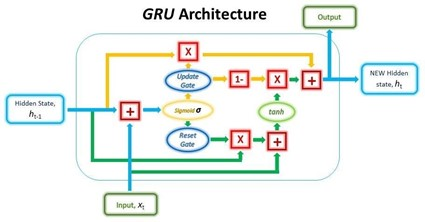
\includegraphics[width=0.80\textwidth]
            		{./Figuras/gru_arch.jpg}
            	
            	\caption{Arquitetura do modelo GRU}
            	\subcaption*{ Fonte:  http://deeplearningbook.com.br/arquitetura-de-redes-neurais-gated-recurrent-unit-gru/} \label{fig:gru-arch}}
            \end{figure}